\chapter{Algorithm}

The time complexity of the algorithm is $O(n)$ with respect to the number of iterations applied and
the number of vertices that make up the sphere, making it suitable for on-the-fly generation and
real-time computer graphics.  In the context of raytracing, the time complexity of the algorithm
becomes linear with respect only to the number of iterations, since the linear complexity of a
simple raytracer with respect to the number of pixels rendered is already built-in.

The algorithm works by generating a randomly oriented plane and splitting the sphere geometry in
two, then applying anti-symmetric transformations to the two hemispheres.  The fact that the two
separate transformations are anti-symmetric ensures that the sphere volume does not diverge out of
control over time, as more and more iterations are applied.

Intuitively, the algorithm can be understood as follows. Note how, for the general case, there is no
additional time complexity for surface points (in the case of raytracing, for example, it could be
argued that, for all practical purposes, there is a one-to-one relationship between pixels and
surface points---this is dealt with during rendering and thus does not need to be taken into account
in the algorithm).

\begin{enumerate}
  \itemsep0em
  \item Begin with a sphere of radius $r$ positioned with its center point at $(0, 0, 0)$.
  \item Select a random normal $\vec{N}$ to represent a plane in $\mathbb{R}^3$.
  \item Let the plane defined by $\vec{N}$ split the sphere in two halves, $S_A$ and $S_B$.
  \item Scale $S_A$ by some factor $k$ where $k\approx 1$, $k\ne 1$.
  \item Scale $S_B$ by the reciprocal, $k^{-1}$.
  \item Repeat from step 2 an arbitrary number of iterations.
\end{enumerate}
\fig{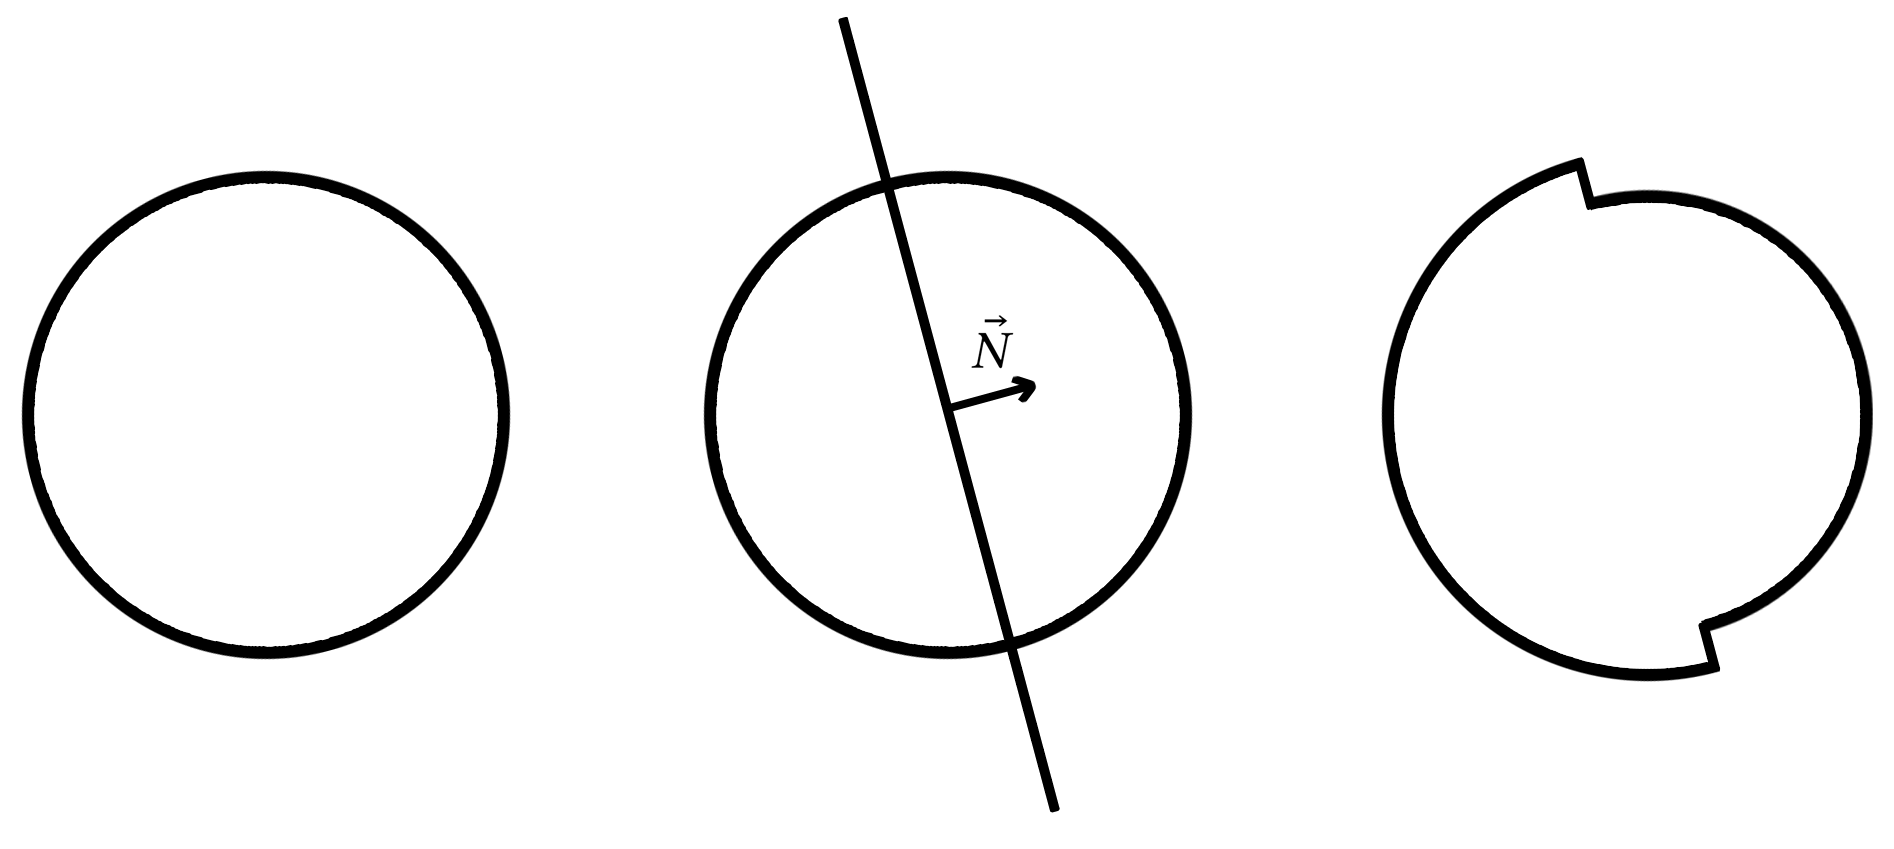
\includegraphics[width=0.8\textwidth]{algorithm-illustration}}{Illustration of a single
  iteration applied to a sphere.}

\noindent When working with triangle-vertex meshes, the algorithm needs to be slightly more specific
and operate on individual points.  The pseudocode below describes one way to implement the algorithm
for triangle-vertex meshes:

\fig{
  \begin{algorithmic}[1]
    \State$\mathit{num\_iterations}\gets 1000$
    \State$k\gets0.99+0.02{\mathit{random()}}$
    \For{$i\gets1$ \textbf{to} $\mathit{num\_iterations}$}
      \State$\vec{N}\gets$ random normal in $\mathbb{R}^3$
      \For{each vertex $p\in\mathbb{R}^3$ in sphere mesh}
        \State$\vec{a}\gets$ vector from center of sphere to $p$
        \State$d\gets\vec{a}\cdot\vec{N}$
        \If{d < 0}
          \State$p'\gets p+k\vec{a}$
        \Else%
          \State$p'\gets p-k\vec{a}$
        \EndIf%
      \EndFor%
    \EndFor%
  \end{algorithmic}
}{Pseudocode for implementing the algorithm.}
